% !TEX root = BA-Bauer.tex

\subsection{Gehäusedesign}
Mit dem Gehäuse wird aus der eher abstrakt wirkenden Platine ein optisch ansprechendes Endprodukt. Wichtig ist nicht nur die Optik, sondern auch das Design in funktioneller Sichtweise. Das beschriebene Platinendesign in Kapitel \ref{sec:PCB-Design} und das 3D-Modell bilden die Basis für die Entwicklung des Gehäuses. Diese können durch die Verbindung von $EAGLE$ mit der 3D-CAD-Software $Fusion360$  der Firma Autodesk direkt virtuell in die Konstruktion eingefügt werden. Damit kann sichergestellt werden, dass z.B. Bohrungen im Gehäuse mit den in der Platine befindlichen übereinstimmen und dass die Bauteile auf der Platine nicht mit dem Gehäuse kollidieren. Die Konstruktion ist auf die Fertigung im 3D-Druckverfahren ausgerichtet, da so in kurzer Zeit Design-Iterationen kostengünstig hergestellt werden können. Bei dem verwendeten Material handelt es sich um den biologisch abbaubaren Kunststoff $Poly-lactid-acid$ (PLA). Er ist einfach zu drucken, nachzubearbeiten, kostengünstig in der Anschaffung und besitzt eine ausreichende Stabilität.\\
Abbildung \ref{fig:Housing-front} und \ref{fig:Housing-back} zeigen das 3D-Modell des Gehäuses, dessen grundsätzliches Design simpel und kompakt ist (15,7\,cm breit, 8,14\,cm tief und 5,25\,cm hoch). Die Breite und Tiefe des Gehäuses werden nahezu komplett von der Platine ausgefüllt. Die Höhe des Gehäuses wird von den XLR-Buchsen vorgegeben und ist daher besonders im vorderen Teil nicht voll ausgenutzt. Bei einer Weiterentwicklung könnte dieser freie Platz für einen integrierten Akku genutzt werden. Der Boden des Gehäuses verläuft parallel zur Platine, damit die eingesteckten Kabel rechtwinklig zur Tischoberfläche verlaufen und sie somit das Gerät durch ihr Eigengewicht nicht zum Kippen bringen. Auf der Oberseite befindet sich ein rechteckiger Ausschnitt für das LCD-Modul, sowie runde Ausschnitte für die LEDs, Taster und den Encoder. Über den LEDs befinden sich weiße Diffusionsscheiben, die das Licht der darunterliegenden LEDs brechen. Somit ist das Leuchten aus größerer Distanz und anderen Blickwinkeln sichtbar. Auf der Rückseite befinden sich runde Ausschnitte für die XLR-Buchsen und eine Vielzahl von Schlitzen, die einen Luftaustausch ermöglichen und einem Hitzestau vorbeugen. Auf der linken Seite befinden sich Ausschnitte für den SD-Kartensteckplatz und den USB-Anschluss.
\begin{figure}[h]
	\begin{minipage}{.45\linewidth}
		\centering
		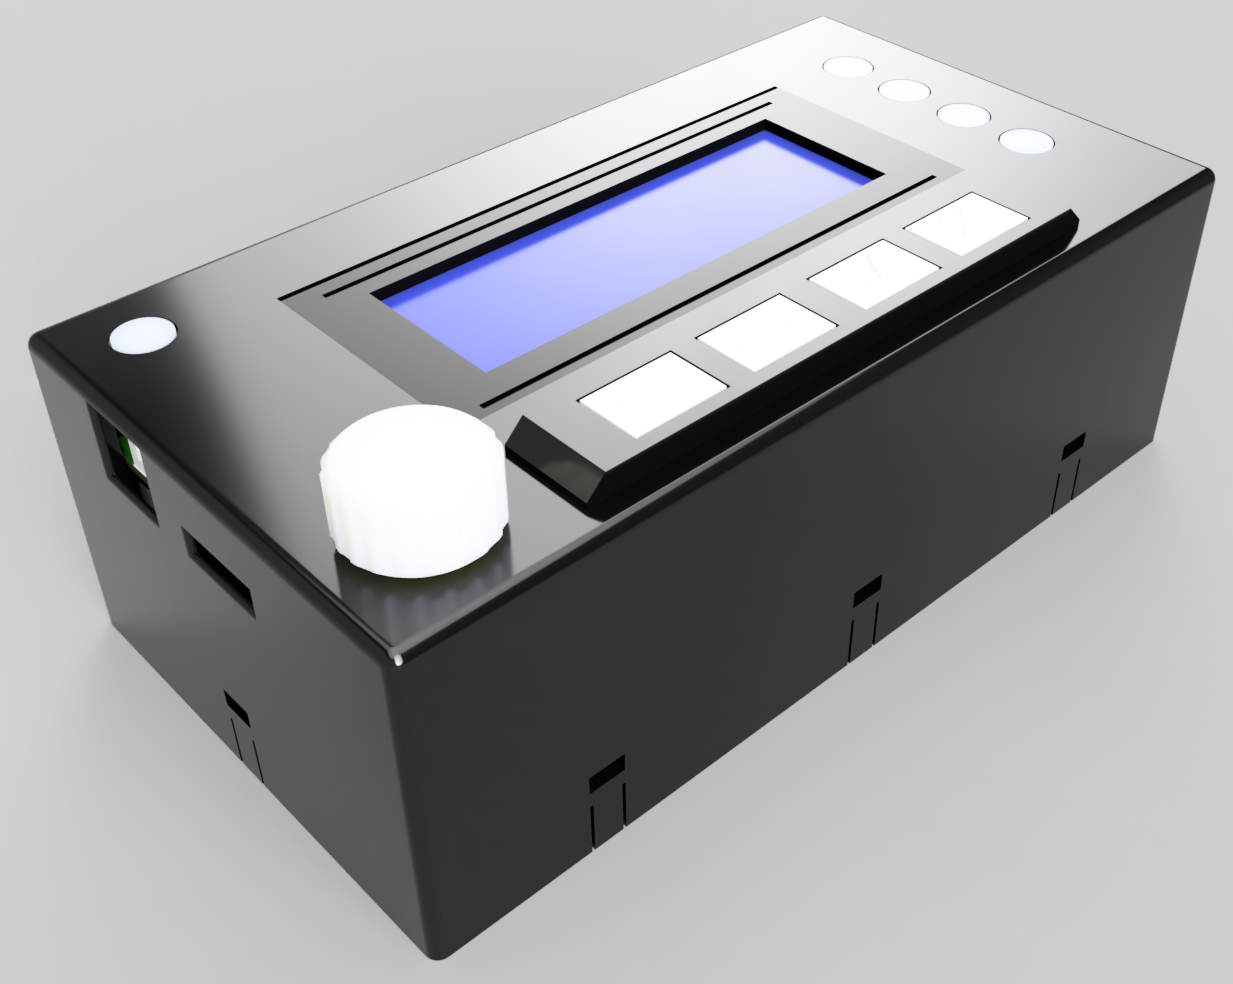
\includegraphics[height=.2\textheight]{Housing-front}
		\caption{Gehäuse 3D-Modell Frontseite}
		\label{fig:Housing-front}
	\end{minipage}
	\hfill
	\begin{minipage}{.45\linewidth}
		\centering
		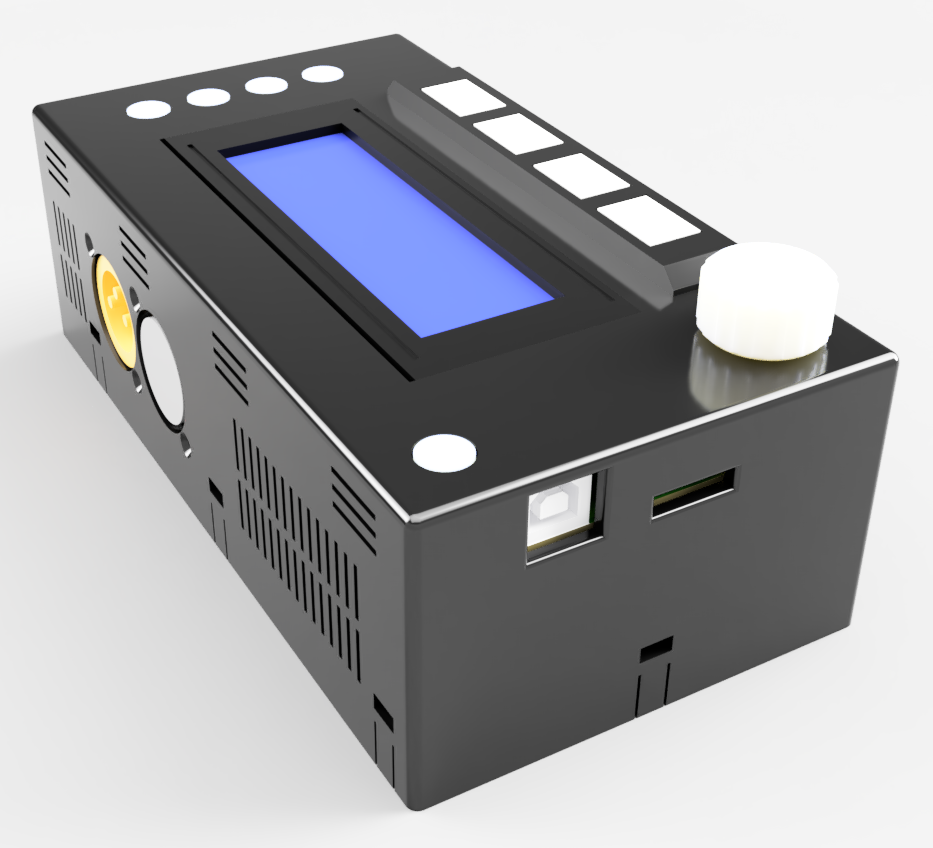
\includegraphics[height=.2\textheight]{Housing-back}
		\caption{Gehäuse 3D-Modell Rückseite}
		\label{fig:Housing-back}
	\end{minipage}
\end{figure}
Die Platine muss ausreichend im Gehäuse befestigt sein, damit sie sich beim Betätigen der Taster nicht kurzzeitig verbiegt. Durch das kurzzeitige Verbiegen wird das Betätigen der Taster erschwert bzw. unmöglich gemacht und die Platine unter Umständen beschädigt. Abbildung \ref{fig:Housing-Befestigung} und \ref{fig:Housing-Befestigung2} zeigen Schnittanalysen des 3D-Modells. Für einen größtmöglichen Halt der Platine im Bereich der Taster wird die Platine in einen Schlitz im Gehäuse eingeführt (rot markiert). Durch den Schlitz wird die Auflagefläche der Platine im Gehäuse erhöht und die durch einen Tastendruck einwirkende Kraft auf sie verteilt. Auf der gegenüberliegenden Seite wird die Platine mit M3-Gewinde-Schrauben befestigt (blau markiert). Dazu befinden sich zylinderförmige Extrusionen an der Oberseite, die mittig eine Bohrung mit einem M3-Gewinde haben. Mit der grün markierten Bohrung wird das LCD-Modul mit den bereits vorhanden Löchern verschraubt. Abstandshalter zwischen LCD-Modul und Platine ermöglichen die Verschraubung von der Unterseite der Platine.
\begin{figure}[h]
	\begin{minipage}{.35\linewidth}
		\centering
		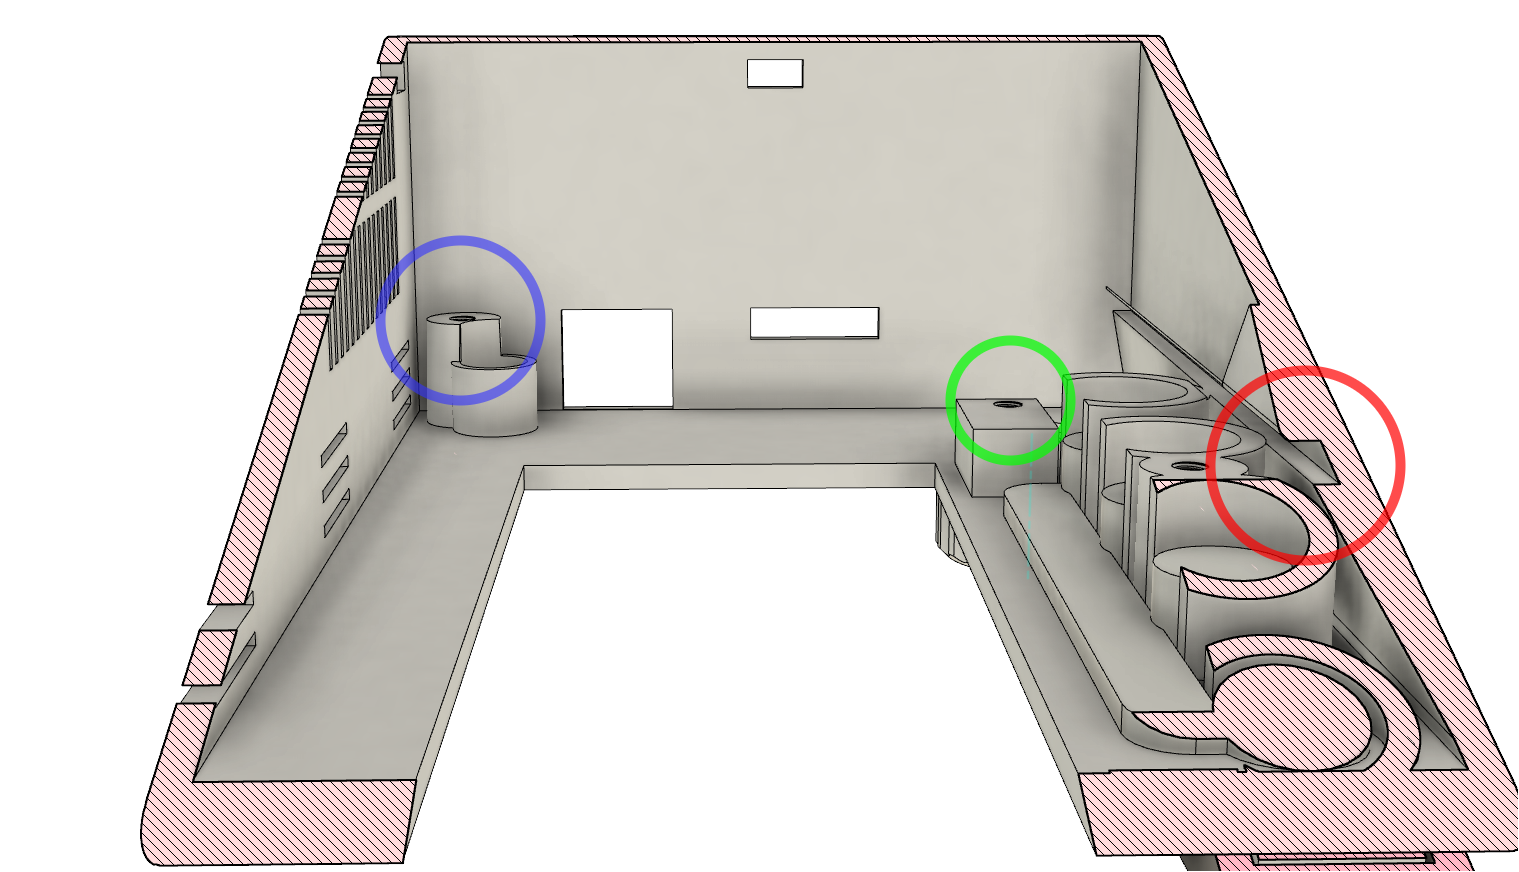
\includegraphics[height=.13\textheight, angle=180]{Housing-Schnitt-Befestigung-mark}
		\caption{Gehäuse Schnitt}
		\label{fig:Housing-Befestigung}
	\end{minipage}
	\hfill
	\begin{minipage}{.55\linewidth}
		\centering
		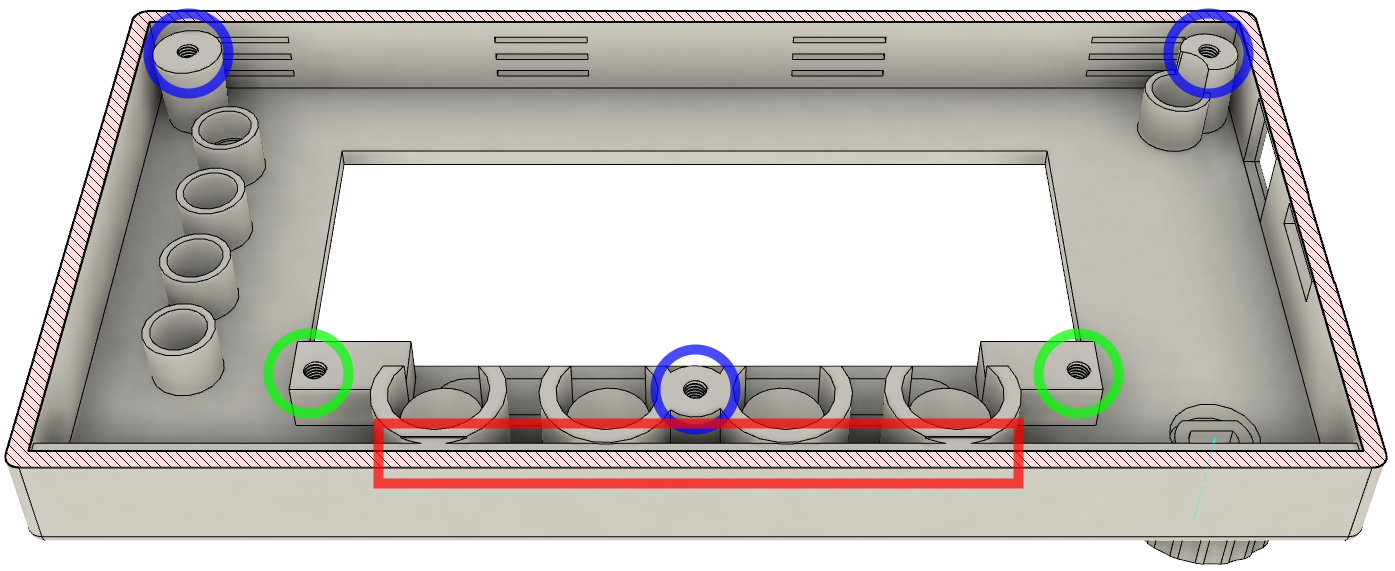
\includegraphics[height=.13\textheight, angle=180]{Housing-Schnitt-Befestigung2-mark}
		\caption{Gehäuse Schnitt Draufsicht}
		\label{fig:Housing-Befestigung2}
	\end{minipage}
\end{figure}
Damit die Platine im Gehäuse platziert und befestigt werden kann, muss das Gehäuse geöffnet werden können. Um bei der Entwicklung möglichst unkompliziert die Platine erreichen zu können, befindet sich ein Clip-Mechanismus an der Unterseite des Gerätes, mit dem der Boden einfach entfernt werden kann. Abbildung \ref{fig:Housing-clip-side} zeigt die Seitenansicht des Mechanismus. In der Oberseite des Gehäuses befinden sich rechteckige Aussparungen, in die die an der Unterseite befindlichen Clips einhaken können. Durch das verwendete 3D-Druckverfahren sind die Clips eine Schwachstelle der Konstruktion, da PLA verhältnismäßig spröde ist und die Clips beim Einhaken in die Aussparungen leicht gebogen werden müssen. Um das Material beim verbiegen weniger zu belasten, sind die Clips bis in den Boden hinein verlängert. Dadurch wird das Material auf eine längere Strecke hinweg gebogen und das Biegemoment somit verteilt.
\begin{figure}[h]
		\begin{minipage}{.45\linewidth}
		\centering
		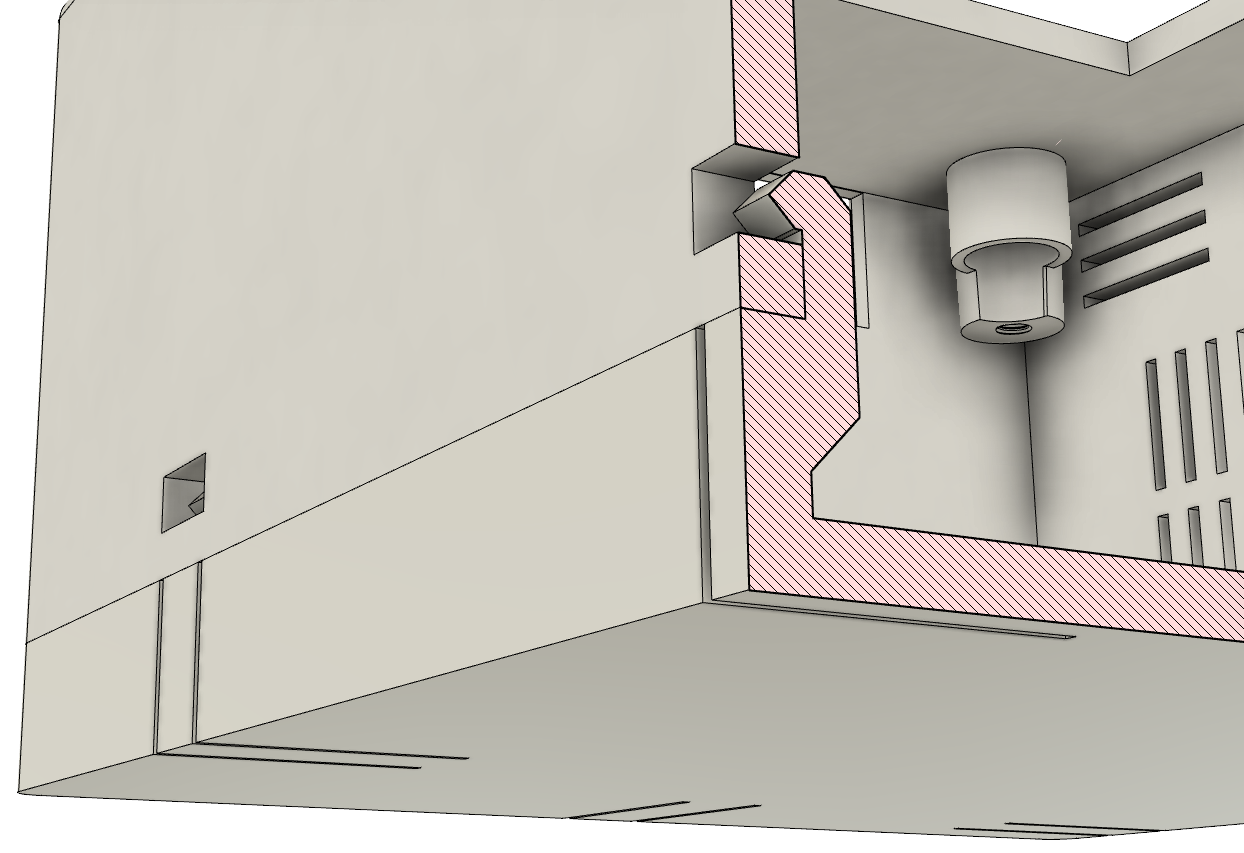
\includegraphics[height=.15\textheight]{Housing-Schnitt-Clip}
		\caption{Gehäuse Clip-Mechanismus Schnittansicht frontal}
		\label{fig:Housing-clip}
	\end{minipage}
	\hfill
	\begin{minipage}{.45\linewidth}
		\centering
		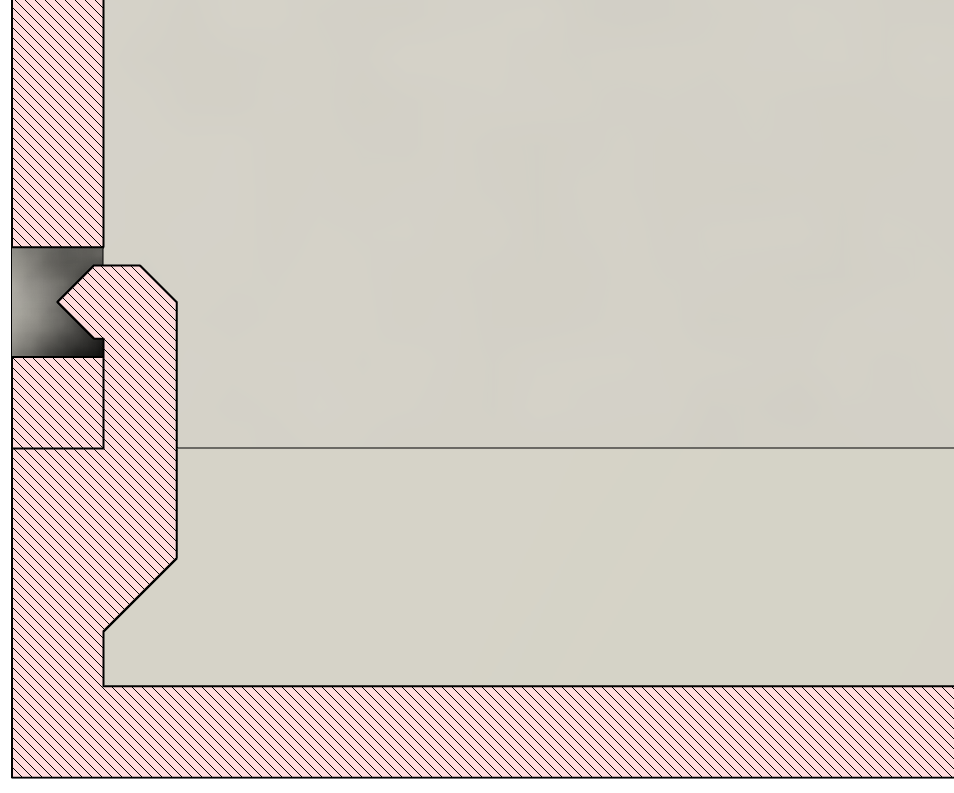
\includegraphics[height=.15\textheight]{Housing-Schnitt-Clip-Seite}
		\caption{Gehäuse Clip-Mechanismus Schnittansicht}
		\label{fig:Housing-clip-side}
	\end{minipage}
\end{figure}\\
Einen wichtigen Bestandteil der Bedienbarkeit stellen die Taster dar. Abbildung \ref{fig:Housing-btn-front} und \ref{fig:Housing-btn} zeigen den Mechanismus zum Betätigen des Tasters als Schnittansicht des 3D-Modells. Die Körper mit der Kennzeichnung 1 sind das Gehäuse an sich, die Taster sind mit 4 gekennzeichnet. Unter den Tastern befindet sich die Platine. Im Gehäuse befinden sich vier nach unten gerichtete Führungen für einen beweglichen Zylinder, welcher mit 3 gekennzeichnet ist. Alle vier Zylinder sind miteinander verbunden, um die Stabilität zu erhöhen und ein Verkanten dieser mit der Führung zu verhindern. Für die Zylinder wird ein gummiartiges Material namens $TPU$ für den 3D-Druck verwendet, wodurch das Klicken des Tasters gedämpft wird. Die für den Benutzer sichtbaren beweglichen Taster-Flächen, gekennzeichnet mit 2, drücken den Zylinder bei einer Betätigung nach unten und diese wiederum betätigen den Taster. Auf den Tasterflächen befinden sich Extrusionen mit der Kennzeichnung der entsprechenden Funktion des jeweiligen Tasters. Dadurch kann der Taster optisch und haptisch wahrgenommen werden, was besonders an Orten mit schlechten Beleuchtungsverhältnissen wichtig ist.
%Formulierung: TPU wegen der Verbindung der Zylinder. Tasterdruck könnte mehrere Tasten betätigen
\begin{figure}[h]
	\begin{minipage}{.45\linewidth}
		\centering
		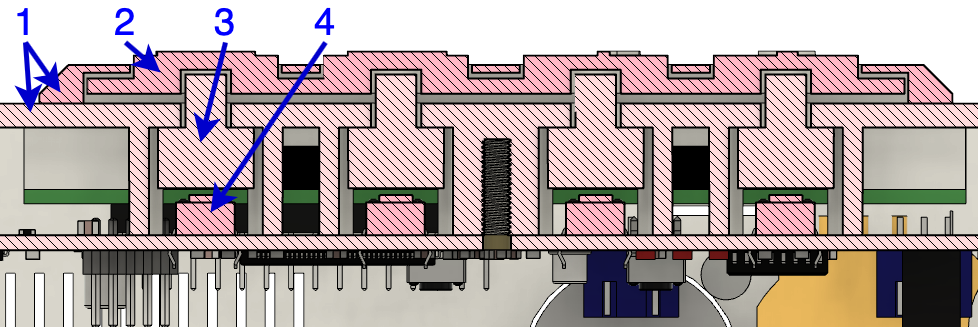
\includegraphics[width=\linewidth]{Housing-Schnitt-Button-front-crop-mark}
		\caption{Gehäuse Clip-Mechanismus}
		\label{fig:Housing-btn-front}
	\end{minipage}
	\hfill
	\begin{minipage}{.45\linewidth}
		\centering
		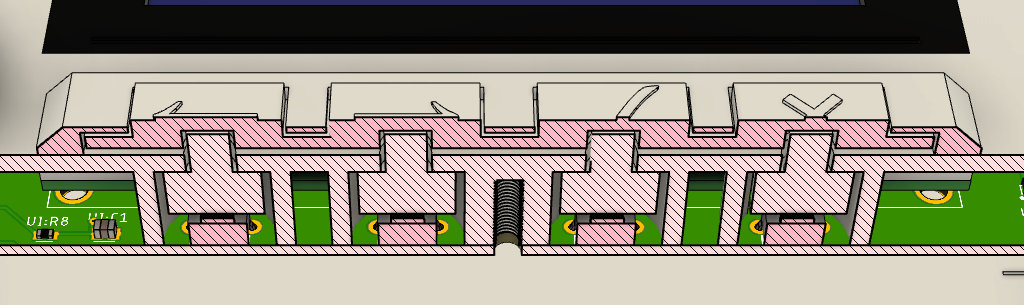
\includegraphics[width=\linewidth]{Housing-Schnitt-Button-crop}
		\caption{Gehäuse Clip-Mechanismus Schnittansicht}
		\label{fig:Housing-btn}
	\end{minipage}
\end{figure}\\
Alle konstruierten Komponenten, sowie das 3D-Modell der Platine befinden sich als $.stl$-Datei im Anhang \ref{CD-Anhang}.\\
\newline
\textbf{Optimierungsmöglichkeiten}\\
Das verwendete Material für das 3D-Druckverfahren ist, wie bereits erwähnt, verhältnismäßig spröde. Aus diesem Grund sind die Wände des Gehäuses dicker Konstruiert, als es für die Herstellung mit einem Spritzgussverfahren mit ABS-Kunststoff notwendig wäre. Durch die Dicke der Wände kann die SD-Karte durch den Schlitz im Gehäuse nur schwer erreicht werden. Durch eine Vergrößerung des Schlitzes oder eine Verringerung der Wanddicke kann dieses Problem gelöst werden. Außerdem ist der Mechanismus für die Taster optimierungsbedürftig. Die Verbindung der Tasterflächen ist zu steif, wodurch beim Betätigen eines Tasters der jeweilige benachbarte Taster betätigt werden kann. Durch die Konstruktion einzelner Tasterflächen für jeden Taster kann das Problem gelöst werden. 